   %\documentclass[wcp,gray]{jmlr} % test grayscale version
\documentclass[wcp]{jmlr}


%% Personnal package
\usepackage{enumerate}
\usepackage{bbold}
\usepackage{wrapfig}


 % The following packages will be automatically loaded:
 % amsmath, amssymb, natbib, graphicx, url, algorithm2e

 %\usepackage{rotating}% for sideways figures and tables
% \usepackage{longtable}% for long tables

 % The booktabs package is used by this sample document
 % (it provides \toprule, \midrule and \bottomrule).
 % Remove the next line if you don't require it.
\usepackage{booktabs}
 % The siunitx package is used by this sample document
 % to align numbers in a column by their decimal point.
 % Remove the next line if you don't require it.
\usepackage[load-configurations=version-1]{siunitx} % newer version
 %\usepackage{siunitx}
\usepackage[utf8]{inputenc}

 % The following command is just for this sample document:
\newcommand{\cs}[1]{\texttt{\char`\\#1}}

% % Define an unnumbered theorem just for this sample document:
%\theorembodyfont{\upshape}
%\theoremheaderfont{\scshape}
%\theorempostheader{:}
%\theoremsep{\newline}
%\newtheorem*{note}{Note}

 % change the arguments, as appropriate, in the following:
\jmlrvolume{1}
\jmlryear{2014}
\jmlrworkshop{\textcolor{red}{Neural Connectomics Workshop}}

% \title[Connectomics challenge]{Inferring neural networks from fluorescent
%                                calcium imaging using partial correlation and
%                                sample weighting \textcolor{red}{plus court} : Simple and robust inference of connectomes using partial correlation coefficients
% ?}

% \title[Inference of connectomes using partial correlation coefficients]{Simple and robust inference of connectomes using partial correlation coefficients}

\title{\textcolor{red}{Simple} connectome inference using partial correlation from imaging calcium signal}


% %%
% Discovery/Infering/Retrieving/... connectomes
% Robust
% Using partial correlation
% [from calcium imaging]


 % Use \Name{Author Name} to specify the name.
 % If the surname contains spaces, enclose the surname
 % in braces, e.g. \Name{John {Smith Jones}} similarly
 % if the name has a "von" part, e.g \Name{Jane {de Winter}}.
 % If the first letter in the forenames is a diacritic
 % enclose the diacritic in braces, e.g. \Name{{\'E}louise Smith}

 % Two authors with the same address
%  \author{\Name{Author Name1\nametag{\thanks{with a note}}} \Email{abc@sample.com}\and
%   \Name{Author Name2} \Email{xyz@sample.com}\\
%   \addr Address}

 % Three or more authors with the same address:
 % \author{ Antonio Sutera %\and
 %         % \Name{Arnaud Joly} \and
 %         % \Name{Vincent Fran\c{c}ois-Lavet} \and
 %         % \Name{Aaron Qiu} \and
 %         % \Name{Gilles Louppe} \and
 %         % \Name{Damien Ernst} \and
 %         % \name{Pierre Geurts}}
 %         }
\author{Antonio Sutera,
        Arnaud Joly,
        Vincent François-Lavet,
        Aaron Qiu, \\
        Gilles Louppe,
        Damien Ernst,
        Pierre Geurts}

 % Authors with different addresses:
 % \author{\Name{Author Name1} \Email{abc@sample.com}\\
 % \addr Address 1
 % \AND
 % \Name{Author Name2} \Email{xyz@sample.com}\\
 % \addr Address 2
 %}

\editor{Editor's name}
 % \editors{List of editors' names}

\begin{document}

\maketitle


\begin{abstract}
Understanding how the brain works is a key
to treat brain disorders such as Parkinson's disease,
epilepsy. Retrieving connectomes, the neurons wiring map, will shed a new
light on the anatomical and functional connectivity of the brain. In the
context of the Connectomics challenge, we propose a simple algorithm made of
four stages, using preprocessing and partial correlation to achieve a network
inference of high quality. An optimized variation of this simple algorithm
is the winning method of the Connectomics Challenge.
We put in perspective our method
with other inference methods such as GTE (\cite{stetter2012model}) and Genie3
(\cite{huynhthu2010inferring}).

% Discussion on the metrics?
%\textcolor{red}{Discussion on the order of the partial correlation}

\end{abstract}

\begin{keywords}
Network inference - Partial correlation - Precision matrix - GENIE3
\end{keywords}


\section{Introduction}\label{sec:intro}

% BG : brain, complex organ
The human brain is a complex biological organ, formed by 100
billions of neurons with 7000 synaptic connections on average.
Cutting edge optical devices delivers in real-time  2-D  images of
the neuronal activity of thousands of neurons through a fluorescent
calcium indicator [todo cite]. Automatic and analytical methods are required to infer
the connectomes from those time series and have to handle several
experimental issues. Some neurons of the network might not be
observed or are confounded with others. The lower device sampling rate with
respect to neuronal activity speed might not allow to distinguish neuron
activation order, especially in highly synchronous activity
[Stetter and in Stetter [20,46,47]] of a large part of the network. Moreover
the fluorescent concentration is highly reactive to a neuron activation or a
spike, but have a slow decay.

% Introduce notation + goal in mathematical score
The connectomes, the neural network, is represented by a (un)directed graph $G = (V, E)$ comprising
a set of nodes $V$ and a set of edges $E \subseteq \left\{(i, j) \in V \times
V\right\}$, (un)ordered pair from $V$.
Each node $i \in V$ represents a neuron, and each edge $(i, j) \in E$
represents a direct link and interactions between neuron $i$ and a neuron $j$.
In the directed graph, each edges also expresses a causal relationship: an
edge $(i, j) \in E$ indicates that the state of neuron $j$ might be caused
by the neuron $i$. The network inference task is set as follows :
\textit{Given the observations $(x^t \in \mathcal{R}^{|V|})_{t=1}^T $
along $T$ periods of time of the $|V|$ neurons, the goal is to infer the
adjacency matrix $A : a_{i,j} = \mathbb{1}((i, j) \in E)$ of the neural network
of graph $G$, where $\mathbb{1}$ is the indicator function.}

The directivity in the network introduce causal relations through neurons. A
directed edge, i.e. $a_{i,j} = 1$ and $a_{j,i} = 0$, means that neuron $i$
causes $j$. The causal mechanism implies that when neuron $i$ is active, also
denoted in this paper as a firing event or a burst, neuron $j$ may be
afterwards activated consequently. Let us notice that neuron $j$ depends on
all its ancestors and its activation may not be as straightforward as we may
think if the causal activation is not systematic (stochastic?). The reciprocal
phenomenon is only possible when the edge is bidirectionnal, i.e. $a_{i,j} =
a_{j,i} = 1$.

% Solution

In this paper, we describe a simple and a theoretically grounded approach
based on partial correlation\footnote{Source code is available at
\url{https://github.com/asutera/kaggle-connectomics}.} to infer the neural
network, which is the winning method of the Connectomics challenge
\footnote{\url{http://connectomics.chalearn.org}}.

\textcolor{red}{It may be useful to rewritte the following lines but I add it to not forget about a plan (request from AQ)}
In section \ref{sec:filter}, we will describe how we filter the fluorescent calcium imaging signal.
In section \ref{sec:inference}, we will characterize our algorithm from a theoretical point of view.
In section \ref{sec:results}, we will present some results and give a critical comparision with other inference methods.
In appendix \ref{app:optimized}, we describe a fully tuned version of our algorithm which has won the Connectomics challenge.



\section{Signal filtering} \label{sec:filter}

Given the image acquisition process, the fluorescent calcium time series
are smoothed using several linear and non linear filters in
order to reduce the imaging process effects. The overall filtering approach
is displayed at Figure \ref{fig:fitlering}.


\begin{figure}[bth]
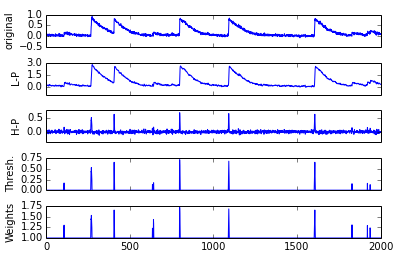
\includegraphics[width=\linewidth]{images/fig_filtering_recut.png}
\caption{Filtering steps. \textcolor{red}{TODO remake in pdf}}
\label{fig:fitlering}
\end{figure}

The raw signal (original signal of Figure \ref{fig:fitlering}) is very noisy
due to light scattering artifacts that ordinarily affects the quality of the
recording (\cite{lichtman2011big}). A low-pass filter is first applied to
filter high frequency noises with one of the following filter designs
\begin{align}
% symmetrical median filter
x^t_i &\leftarrow x^{t-1}_i + x^{t}_i + x^{t+1}_i \label{eq:symetric-median}, \\
% asymmetrical weighted median
x^t_i &\leftarrow 0.4 x^{t-3}_i + 0.6 x^{t-2}_i + 0.8 x^{t-1}_i + x_{t}^i.
\label{eq:weighted-asymetric-median}.
\end{align}

A neuron spike lasts on average $1ms$ to $2ms$, while current optical
device have a time resolution of $20ms$. Considering the short delay for a
communication between neurons and slow decay of fluorescence signal, we
can filter low frequencies through an asymmetrical discrete derivative filter
\begin{align}
x^{t,d}_{i} &\leftarrow x^{t}_i - x_{t-1}^i.
\end{align}
When slow signals variations are filtered (H-P signals of figure
\ref{fig:filtering}), only remains spike positions.
\textcolor{red}{Pourquoi sur la figure, on a pas de signal avec une dérivée
                négative?}


By nature, the firing event is really fast and in order to
retrieve the connectivity from them, it is necessary to link a burst to a
couple of timesteps (ideally one). The small decay for the fluorescent calcium
indicator implies a signal
variation during a long time interval. Firing event are represented by strong
variations in the neuron activity. Therefore we apply a hard-tresholding
filter
\begin{align}
x^{t,d}_i &\leftarrow x^{t,d}_i \mathbb{1}(x^{t,d}_i \geq \tau)
\end{align}
where the threshold $\tau$ should be taken positive and non-close to zero to
respectively only keep rising edges and strong variations.


As a result, we get a binary-like signal with the true activity when a burst
happens and with a true zero when the neuron is inactive.


Then we apply on the entire signal a non-linear filter based on the current
activity of the systems in order to favor the association measure inversely
proportional to the number of neurons firing together: $ x^{t,w}_i  =
(x^{t,d}_i + 1 )^{1 + \frac{1}{act_t}}$ where $act_t = \sum_{j} x^{t,d}_j$ is
the activity of all neurons at time $t$. When too much neurons are firing
together, i.e. in case of a network burst, it is almost impossible to retrieve
direct relationships: all neurons seem to be directly connected to each other.
By favoring the association measure when the activity is low, we expect to
retrieve a pair of neurons that are really directly connected together. In
concrete terms, as it can be verified on \textit{fig 1}, peak intensity may
change in function of the activity of all neurons but the number and the
locations of peaks is not modified.


\section{Network inference through weighted average partial correlation
            coefficients}
\label{sec:inference}

Let us denote the fluorescence calcium indicators of all neuron
as a set of random variables $X = \left\{X_1, \ldots, X_{|V|}\right\}$, which follows
a joint probability distribution $p_\mathcal{X}$, and by
$X^{-i,j}$ the set of all variables except $X_i$ and $X_j$.
Two random variables $X_i$ and $X_j$ are said to be conditionally independent
to a (possibly empty) set of random variables $Z$, denoted by $X_i \perp X_j | Z$,
if the joint conditional probability distribution factorizes
$p_{\mathcal{X}_i, \mathcal{X}_j|\mathcal{Z}} = p_{\mathcal{X}_i|\mathcal{Z}}
p_{\mathcal{X}_j|\mathcal{Z}}$.  The inference of the undirected network
can be formulated as inferring conditional dependences
$X_i \not\perp X_j | X^{-i,j}$ between all pairs $i$ and $j$ of fluorescence
signals, in other words the inferred network will be
$\hat{A}: \hat{a}_{i,j} = \mathbb{1}(X_i \not\perp X_j | X^{-i,j}), \forall i, j \in V$.


Since all neurons are assumed to form a connected graph, we
have by construction $X_i \not\perp X_j$. However, two random variables $A$ and $B$ might be
dependent taken alone ($A \not\perp B$), but not once we observe the set  $C$
of all other variables ($A \perp B | C$). The conditioning over all other
random variables $X^{-i,j}$ is thus necessary to avoid predicting an edge when
two neurons are not directly connected.

If the random variables $X$ follows a joint Gaussian distribution
$p_\mathcal{X} \sim \mathcal{N}(\mu; \Sigma)$ of mean vector $\mu$ and
covariance matrix $\Sigma$, we have the conditional independence
$X_i \perp X_j | X^{-i,j}$ if the partial correlation coefficient
\[
\rho_{X_i, X_j | X^{-i,j}}
= \frac{\Sigma^{-1}_{ij}}{\sqrt{\Sigma^{-1}_{ii} \Sigma^{-1}_{jj}}}
\]
is equal to zero (\cite{koller2009probabilistic}). The partial correlation gives
a connectivity score
$\hat{A}: \hat{a}_{i,j} = \rho_{X_i, X_j | X^{-i,j}}, \forall i, j \in V$ between all
pairs of neuron $i$ and $j$. One could retrieve an estimated graph by thresholding
the matrix $\hat{A}$.
Similarly, we also have $X_i \perp X_j$ if the Pearson correlation
coefficient
\[
\rho_{X_i,X_j} = \frac{\Sigma_{ij}}{\sqrt{\Sigma_{ii}
\Sigma_{jj}}}
\]
is equal to zero.

% Speak about why averaging
The quality of the signal filtering and network inference depends on
good hyper-parameter selection, which are themselves dependent on the properties
of the targeted network and measurement conditions, e.g. signal to noise ratio.
In order to improve robustness, a weighted average of partial correlation
matrices was estimated from the time series by varying the hard-threshold value
$\tau$ and the design of the low-pass filter (mentionned in section \ref{sec:filter} and appendix \ref{app:optimized}).


% Introduce a custom solution to make the Y matrix asymmetric
% Introduce directivity
\textcolor{red}{Est-ce qu'on ne le ferait pas passer dans l'appendice B? Ou du moins l'équation?}
Since partial correlation is a symmetric measure, the causal mechanism behind the
interaction ($A$ directly causes $B$, $B$ directly causes $A$ or both) can not
be directly inferred\footnote{Also note that two other causal mechanisms might be
implied while having a non-zero partial coefficient: (i) a pair of variables
is induced by a common (hidden) variable; (ii) $A$ (respectively $B$) is
conditionally correlated to a hidden variable affecting $B$ (resp. $A$)
\cite{de2004discovery}.}.
In order to retrieve causal information, we developed an
heuristics based on the following observation. The rise of fluorescence
indicates the activation of a neuron $i$. If a neuron $j$ have also
an increased of fluorescence after a slight delay, this could have been
caused by the neuron $i$. Thus, we count whenever
such events occurred between consecutive time steps
\[
\hat{Z}: z_{ij} = \sum_{t=1}^{T - 1}
    \mathbb{1}(x_j^{t+1} - x_i^t \in \left[f_1, f_2 \right]) -
    \mathbb{1}(x_i^{t+1} - x_j^t \in \left[f_1, f_2 \right]), \forall i, j \in V
\]
where $f_1$ and $f_2$ are parameters of the method.
Finally, the weighted average of correlation matrices is combined with $Z$ such
that $Z$ has a contribution of $0.3\%$ to the prediction of an edge.


\section{Experiments}
\label{sec:results}

% Datasets
To assess our method, we have used four datasets provided by the organizers
of the Connectomics challenge : \textit{normal-1, normal-2, normal-3, normal-4}.
Those datasets are time series of size $T=179500$ of image calcium from simulated
neuronal networks (\cite{stetter2012model}) with $|V|=1000$ neurons. The networks
to inferred have around 15000 edges and are similar to those
used to rank challenge participants.

% Metrics : ROC AUC and AUPRC
In supervised learning terms, the network inference task can be viewed as a
binary classification task where one has to correctly classify the presence
or the absence of edges of the graph. We assess the accuracy of the
network inference method using the area under the ROC curve (AUROC)
and the area under the precision-recall curve (AUPRC)
(\cite{schrynemackers2013protocols}). Since neurons are not self-connected
($(i, i) \not \in E, \forall i \in V$) and some inference methods could
give maximal scores to the diagonal of $\hat{A}$, e.g. Pearson
correlation, we set those elements to the minimum of $\hat{A}$ prior
assessment.


% TODO
%   - discussions about the results
%   - discussions about the metrics (Gilles' text)

% For the directory method, only filters defined by Equations
% \ref{eq:low-pass}, \ref{eq:high-pass} and \ref{eq:hard-treshold-filter} were
% used.


% Dummy classifier?


% GTE : Explaning the method (default parameters!)

% Explaining the method (thèse de Gilles)
% Genie3 : better in auprc while worse in auroc than GTE. Why?
% Genie3 : "Conditioning" better and better but need a lot of trees
% Correlation : Already give good results

% Partial correlation : Obvious improvements (both metric) because of the conditioning

% Directivity : ?


%Opt: obviously when parameters are tuned/optimized, it's slightly better --> see appendix for a full description of the method
% Avg.: Averaging over the threholds and L-P filters improves a lot both metrics.

GTE is a method which characterizes a relationship between neurons by an
estimation of the generalized transfer entropy (\cite{stetter2012model}). The
goal of this method tries to see if the next time step value is better from
the previous values of this time series or from time series of other neurons.

GENIE3 is a tree-based method which sees the network inference problem as $p$,
the number of variables, independent supervised learning problems (todo cite:
Irrthum?Van Anh?Pierre?). Formally, each sub-problem consists in the
prediction of one variable, the target, from the remaining $p-1$ variables.
This method uses random forests to estimate the target variable and variable
importances can be derived to estimate the adjacency matrix $A$ (see (todo
cite) for a more detailed description of the inference method).

At first sight, it appears on \textit{Table 1} that partial correlation
methods outperform other methods. Two main reasons may explain this method
hierarchy. First, the quality of the infered network seems related to the
conditioning part of the method. In every method except with partial
correlation, indirect links are confounded with direct links.  Secondly, the
gaussian assumption seems verified and thus linear method appears to be
competitive, e.g. the method correlation already gives good results, with a
non-linear method such as GENIE3.

% Discussion about


\begin{table}[tbh]
\centering
\caption{TODO}
\begin{tabular}{@{}l *{8}{c}@{}}
\toprule
  & \multicolumn{4}{c}{AUROC} & \multicolumn{4}{c}{AUPRC} \\
\cmidrule(r){2-5}\cmidrule(r){6-9}
Methods $\backslash$ normal- & 1 & 2 & 3 & 4 & 1 & 2 & 3 & 4 \\
\midrule
GENIE3                 & & & & & & & & \\
Directivity \textcolor{red}{appendix?} & 0.535 & 0.526 & 0.533 & 0.535 & 0.012 & 0.012 & 0.012 & 0.012 \\
Correlation            & 0.886 & 0.884 & 0.891 & 0.877 & 0.153 & 0.145 & 0.170 & 0.132 \\
GTE                    & 0.890 & 0.893 & 0.894 & 0.873 & 0.171 & 0.174 & 0.197 & 0.142 \\
Partial correlation    & 0.930 &  0.927 &  0.926 &  0.923& 0.363  & 0.347 &  0.346 & 0.328 \\
Partial correlation (opt.) & 0.932 & 0.931 & 0.930 & 0.928 & 0.364 & 0.366 & 0.359 & 0.344 \\
Our approach (opt. \& avg.)    & 0.943 & 0.942 & 0.942 & 0.939 & 0.403 & 0.404 & 0.398 & 0.388 \\
Our approach + dir  \textcolor{red}{appendix?}   & 0.944 & 0.943 & 0.942 & 0.940 & 0.404 & 0.405 & 0.399 & 0.389 \\
\bottomrule
\end{tabular}
\end{table}

\begin{table}[tbh]
\centering
\caption{TODO}
\begin{tabular}{@{}l *{8}{c}@{}}
\toprule
  & \multicolumn{4}{c}{AUROC} & \multicolumn{4}{c}{AUPRC} \\
\cmidrule(r){2-5}\cmidrule(r){6-9}
Methods $\backslash$ normal- & 1 & 2 & 3 & 4 & 1 & 2 & 3 & 4 \\
\midrule
No  filtering       & 0.777 & 0.767 & 0.772 & 0.774 & 0.070 & 0.064 & 0.068 & 0.072\\
P                   & 0.925 & 0.925 & 0.924 & 0.923 & 0.322 & 0.324 & 0.323 & 0.312\\
P + W               & 0.931 & 0.930 & 0.928 & 0.927 & 0.333 & 0.334 & 0.327 & 0.313\\
P + W + PCA         & 0.932 & 0.931 & 0.930 & 0.928 & 0.364 & 0.366 & 0.359 & 0.344\\
Averaging           & 0.943 & 0.942 & 0.942 & 0.939 & 0.403 & 0.404 & 0.398 & 0.388\\
Averaging + Directivity & 0.944 & 0.943 & 0.942 & 0.940 & 0.404 & 0.405 & 0.399 & 0.389\\
\bottomrule
\end{tabular}
\end{table}





\section{Conclusion}

In previous study \cite{shipley2002cause}, it has been suggested to
consider correlation coefficients of all possible orders,
i.e. conditioned on every subsets of the set of $p-2$ other variables. This
would take into account multiple indirect paths between a given pair of
variables.

% Possible extensions
% partial autocorrelation function (sometimes "partial correlation function")
% conditional independence test
% Speak about the complexity and parallelization of the methods




\begin{scriptsize}

\paragraph{Acknowledgements.} A. Joly and G. Louppe are research fellows of
the FNRS, Belgium.  A. Sutera is  is recipient of
a F.R.I.A. fellowship of F.R.S.-FNRS, Belgium.
This work is supported by PASCAL2 and the IUAP DYSCO, initiated by the
Belgian State, Science Policy Office.

\end{scriptsize}

\newpage
\clearpage

% We allow the bibliography to be added on top of the 6 pages.
% Supplementary material may be added in the form or a URL pointed to from
% the paper.
\bibliography{references}

\newpage
\clearpage

\appendix


\section{An optimized version of the algorithm to win the challenge}
\label{app:optimized}


The algorithm propose in sections \ref{sec:filter} and \ref{sec:inference} has been optimized at its extreme limit to win the challenge. In this section, we will describe the full tuned algorithm and present some results.

Note that our parameter tuning was mainly
done on the \textit{normal-1} dataset and partly on \textit{normal-4} dataset,
therefore it may justify why these networks are better retrieved despite the
fact that some might be simpler to infer.



\section{Supplementary results}

\begin{table}[htbp]
\centering
\caption{Correlation (ROC). Improvement of each stage of our approach. Note that we choose the
         \textit{best} threshold (\textcolor{red}{for now 0.11}) for stages 1 to 4.}
\begin{tabular}{*{5}{l}}
\toprule
Stage               & normal-1 & normal-2 & normal-3 & normal-4 \\
\midrule
Nothing             & 0.681 & 0.699 & 0.683 & 0.681\\
Weights             & 0.695 & 0.713 & 0.697 & 0.694\\
H-T                 & 0.876 & 0.873 & 0.877 & 0.869\\
H-T + Weights       & 0.886 & 0.884 & 0.891 & 0.877\\
P-P                 & 0.857 & 0.850 & 0.843 & 0.832\\
P-P + Weights       & 0.826 & 0.823 & 0.817 & 0.799\\
\bottomrule
\end{tabular}
\end{table}

\begin{table}[htbp]
\centering
\caption{Correlation (P-R). Improvement of each stage of our approach. Note that we choose the
         \textit{best} threshold (\textcolor{red}{for now 0.11}) for stages 1 to 4.}
\begin{tabular}{*{5}{l}}
\toprule
Stage               & normal-1 & normal-2 & normal-3 & normal-4 \\
\midrule
Nothing             & 0.028 & 0.028 & 0.025 & 0.026\\
Weights             & 0.031 & 0.030 & 0.027 & 0.028\\
H-T                 & 0.143 & 0.128 & 0.150 & 0.129\\
H-T + Weights       & 0.153 & 0.145 & 0.170 & 0.132\\
P-P                 & 0.100 & 0.087 & 0.079 & 0.083\\
P-P + Weights       & 0.079 & 0.071 & 0.067 & 0.064\\
\bottomrule
\end{tabular}
\end{table}

\begin{table}[htb]
\centering
\caption{Comparison (P-R) with other methods (for now, $t = 0.11$)}
\begin{tabular}{*{5}{l}}
\toprule
Methods             & normal-1 & normal-2 & normal-3 & normal-4 \\
\midrule
Correlation (best)         & 0.153 & 0.145 & 0.170 & 0.132 \\
Partial correlation (best) & 0.364 & 0.366 & 0.359 & 0.344 \\
Our approach (best)        & 0.403 & 0.404 & 0.398 & 0.388 \\
GENIE3                     & & & & \\
GTE                        & 0.171 & 0.174 & 0.197 & 0.142 \\
Directivity                & 0.012 & 0.012 & 0.012 & 0.012 \\
Our approach + dir         & 0.404 & 0.405 & 0.399 & 0.389 \\
\bottomrule
\end{tabular}
\end{table}

\begin{table}[htb]
\centering
\caption{Inverse correlation (ROC). Improvement of each stage of our approach. Note that we choose the
         \textit{best} threshold (\textcolor{red}{for now 0.11}) for stages 1 to 4.}
\begin{tabular}{*{5}{l}}
\toprule
Stage               & normal-1 & normal-2 & normal-3 & normal-4 \\
\midrule
Nothing             & 0.777 & 0.767 & 0.772 & 0.774 \\
PCA                 & 0.780 & 0.770 & 0.776 & 0.777 \\
Weights             & 0.780 & 0.769 & 0.776 & 0.777 \\
Weights + PCA       & 0.783 & 0.772 & 0.779 & 0.780 \\
H-T                 & 0.893 & 0.891 & 0.891 & 0.886 \\
H-T + PCA           & 0.894 & 0.892 & 0.891 & 0.886 \\
H-T + Weights       & 0.899 & 0.897 & 0.896 & 0.891 \\
H-T + Weights + PCA & 0.900 & 0.898 & 0.896 & 0.892 \\
P-P                 & 0.925 & 0.925 & 0.924 & 0.923 \\
P-P + PCA           & 0.926 & 0.926 & 0.925 & 0.923 \\
P-P + Weights       & 0.931 & 0.930 & 0.928 & 0.927 \\
P-P + Weights + PCA & 0.932 & 0.931 & 0.930 & 0.928 \\
Averaging (PCA)     & 0.943 & 0.942 & 0.942 & 0.939 \\
Stacking            & 0.944 & 0.943 & 0.942 & 0.940 \\
\bottomrule
\end{tabular}
\end{table}

\begin{table}[htb]
\centering
\caption{Inverse correlation (P-R). Improvement of each stage of our approach. Note that we choose the
         \textit{best} threshold (\textcolor{red}{for now 0.11}) for stages 1 to 4.}
\begin{tabular}{*{5}{l}}
\toprule
Stage               & normal-1 & normal-2 & normal-3 & normal-4 \\
\midrule
Nothing             & 0.070 & 0.064 & 0.068 & 0.072\\
PCA                 & 0.076 & 0.070 & 0.075 & 0.079\\
Weights             & 0.074 & 0.067 & 0.072 & 0.076\\
Weights + PCA       & 0.080 & 0.073 & 0.079 & 0.083\\
H-T                 & 0.264 & 0.260 & 0.269 & 0.241\\
H-T + PCA           & 0.266 & 0.263 & 0.273 & 0.244\\
H-T + Weights       & 0.280 & 0.273 & 0.281 & 0.251\\
H-T + Weights + PCA & 0.284 & 0.278 & 0.285 & 0.255\\
P-P                 & 0.322 & 0.324 & 0.323 & 0.312\\
P-P + PCA           & 0.347 & 0.352 & 0.355 & 0.341\\
P-P + Weights       & 0.333 & 0.334 & 0.327 & 0.313\\
P-P + Weights + PCA & 0.364 & 0.366 & 0.359 & 0.344\\
Averaging           & 0.403 & 0.404 & 0.398 & 0.388\\
Stacking            & 0.404 & 0.405 & 0.399 & 0.389\\
\bottomrule
\end{tabular}
\end{table}



%% Talk about filters future and past

\end{document}

